\PassOptionsToPackage{table}{xcolor}
\documentclass[hyperref={colorlinks},aspectratio=169]{beamer}
\usepackage{amsmath,amssymb,amsthm,booktabs,tikz}
\usepackage[final]{microtype}
\usepackage{libertine}
\usepackage[varqu]{zi4}
\usepackage[libertine]{newtxmath}
\usepackage[T1]{fontenc}
\usepackage[utf8]{inputenc}
\usepackage{multirow,tabto,siunitx}

% Seven colors safe for use color blindness.
% Colors taken from doi:10.1038/nmeth.1618.
\definecolor{cbOrange}{RGB}{230,159,0}
\definecolor{cbSkyBlue}{RGB}{86,180,233}
\definecolor{cbBluishGreen}{RGB}{0,158,115}
\definecolor{cbBlue}{RGB}{0,114,178}
\definecolor{cbVermillion}{RGB}{213,94,0}
\definecolor{cbReddischPurple}{RGB}{204,121,167}
\definecolor{cbYellow}{RGB}{240,228,66}


\newcommand{\At}[1]{\texttt{@#1}}
\newcommand{\Null}{\texttt{@null}}


%% Tikz
\usepackage{tikz}
\usetikzlibrary{arrows.meta,calc,decorations.pathreplacing,shapes.geometric,shapes.multipart,overlay-beamer-styles}
\tikzset{
    >=Stealth,
    dot/.style={circle,scale=0.25,draw=black,fill=black},
    every node/.append style={align=center,font=\strut},
    every node part/.append style={align=center},
    lnode/.style={rectangle split,rectangle split parts=2,font=\strut,rectangle split part fill={black!10,cbYellow!10},rectangle split part align={center}},
    hlisted/.style={right,rectangle split,rectangle split,draw,rectangle split parts=#1,font=\strut,rectangle split part fill={black!10},rectangle split part align={center},text width=0.5cm},
}

\begin{document}

\begin{frame}
        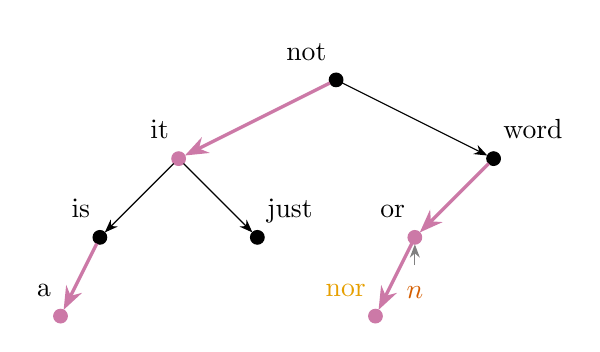
\begin{tikzpicture}
                \node[dot] (p) at (0, 0)       {};
                \node[dot,cbReddischPurple] (l) at (-2, -1)     {}  edge[<-,very thick,cbReddischPurple] (p);
                \node[dot] (ll) at (-3, -2)  {}  edge[<-] (l);
                \node[dot,cbReddischPurple] (lll) at (-3.5, -3) {}  edge[<-,very thick,cbReddischPurple] (ll);
                \node[dot] (lr) at (-1, -2)  {}  edge[<-] (l);



                \node[above left] at (p)  {not};
                \node[above left] at (l)  {it};
                \node[above left] at (ll) {is};
                \node[above left] at (lll) {a};
                \node[above right] at (lr) {just};

                \node[dot] (r) at ( 2, -1)     {}  edge[<-] (p);
                \node[dot,cbReddischPurple] (rl) at ( 1, -2)  {}  edge[<-,very thick,cbReddischPurple] (r);
                \node[above right] at (r)  {word};
                \node[above left] at (rl) {or};
                \node[below=10pt,cbVermillion] at (rl) {$n$} edge[->,black!50] (rl);
                \node[dot,cbReddischPurple] (rll) at (0.5, -3) {} edge[<-,very thick,cbReddischPurple] (rl);
                \node[above left,cbOrange] at (rll) {nor};
        \end{tikzpicture}
\end{frame}

\begin{frame}
            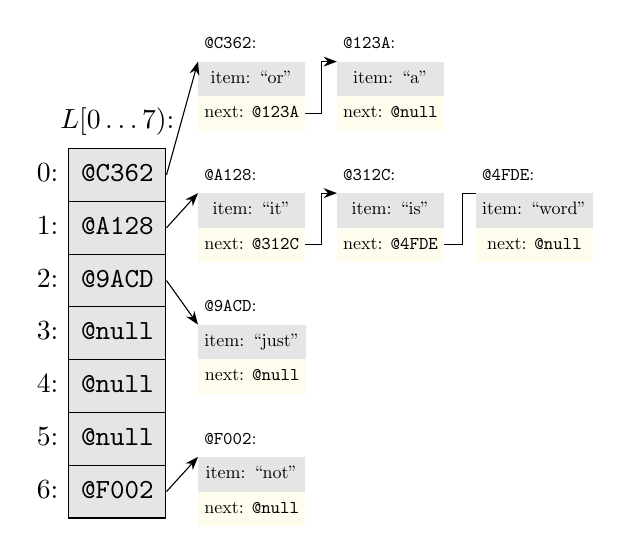
\begin{tikzpicture}
                \node[hlisted=7,text width=1cm] (ar) {
                \At{C362}
                \nodepart{two}\At{A128}
                \nodepart{three}\At{9ACD}
                \nodepart{four}\Null{}
                \nodepart{five}\Null{}
                \nodepart{six}\Null{}
                \nodepart{seven}\At{F002}};
                
                \node[above] at (ar.north) {$L[0\dots7)$:};
                \node[left] at (ar.one west) {0:};
                \node[left] at (ar.two west) {1:};
                \node[left] at (ar.three west) {2:};
                \node[left] at (ar.four west) {3:};
                \node[left] at (ar.five west) {4:};
                \node[left] at (ar.six west) {5:};
                \node[left] at (ar.seven west) {6:};
        \node[lnode,right=0.4cm,yshift=-1cm,scale=0.65] (n4) at (ar.three east) {item: ``{just}''\nodepart{two}next: \Null};
        \node[above right,scale=0.65] at (n4.north west) {\At{9ACD}:};
        \path (ar.three east) edge[->] (n4.north west);

        \node[lnode,right=0.4cm,yshift=1cm,scale=0.65] (n5) at (ar.one east) {item: ``{or}''\nodepart{two}next: \At{123A}};
        \node[above right,scale=0.65] at (n5.north west) {\At{C362}:};
        \path (ar.one east) edge[->] (n5.north west);
                            
        \node[lnode,right=0.4cm,scale=0.65] (n1) at (n5.east) {item: ``a''\nodepart{two}next: \Null};
        \node[above right,scale=0.65] at (n1.north west) {\At{123A}:};
        \draw[->] (n5.two east) -| ($(n5.text split)!0.5!(n1.text split)$) |- (n1.north west);

        \node[lnode,right=0.4cm,scale=0.65] (n6) at (ar.two east) {item: ``{it}''\nodepart{two}next: \At{312C}};
        \node[above right,scale=0.65] at (n6.north west) {\At{A128}:};
        \path (ar.two east) edge[->] (n6.north west);

        \node[lnode,right=0.4cm,scale=0.65] (n3) at (n6.east) {item: ``{is}''\nodepart{two}next: \At{4FDE}};
        \node[above right,scale=0.65] at (n3.north west) {\At{312C}:};
        \draw[->] (n6.two east) -| ($(n6.text split)!0.5!(n3.text split)$) |- (n3.north west);

        \node[lnode,right=0.4cm,scale=0.65] (n2) at (n3.east) {item: ``word''\nodepart{two}next: \Null};
        \node[above right,scale=0.65] at (n2.north west) {\At{4FDE}:};
        \draw (n3.two east) -| ($(n3.text split)!0.5!(n2.text split)$) |- (n2.north west);


        \node[lnode,right=0.4cm,scale=0.65] (n7) at (ar.seven east) {item: ``{not}''\nodepart{two}next: \Null};
        \node[above right,scale=0.65] at (n7.north west) {\At{F002}:};
        \path (ar.seven east) edge[->] (n7.north west);
    \end{tikzpicture}
\end{frame}


\end{document}